% -----------------------------------------------
% Template for ISMIR Papers
% 2021 version, based on previous ISMIR templates

% Requirements :
% * 6+n page length maximum
% * 10MB maximum file size
% * Copyright note must appear in the bottom left corner of first page
% * Clearer statement about citing own work in anonymized submission
% (see conference website for additional details)
% -----------------------------------------------

\documentclass{article}
\usepackage[T1]{fontenc} % add special characters (e.g., umlaute)
\usepackage[utf8]{inputenc} % set utf-8 as default input encoding
\usepackage{ismir,amsmath,cite,url}
\usepackage{float}
\usepackage{amssymb}
\usepackage[ruled]{algorithm2e}
\usepackage{cleveref}
\crefrangeformat{equation}{Eq.~(#3#1#4) to~(#5#2#6)}
\Crefrangeformat{equation}{Equations~(#3#1#4) to~(#5#2#6)}
\usepackage{graphicx}
\usepackage[skip=0.2\baselineskip]{caption}
\usepackage{subcaption}
\usepackage{color}
\usepackage{multirow}
\usepackage{enumitem}
\usepackage{tablefootnote}
\usepackage{dblfloatfix}


\usepackage{lineno}
\linenumbers

% Title. Please use IEEE-compliant title case when specifying the title here,
% as it has implications for the copyright notice
% -----
\title{The power of deep without going deep? A study of HDPGMM music representation learning}

% Note: Please do NOT use \thanks or a \footnote in any of the author markup

% Single address
% To use with only one author or several with the same address
% ---------------
%\oneauthor
% {Names should be omitted for double-blind reviewing}
% {Affiliations should be omitted for double-blind reviewing}

% Two addresses
% --------------
%\twoauthors
%  {First author} {School \\ Department}
%  {Second author} {Company \\ Address}

% Three addresses
% --------------\input{ISMIR2021_paper.tex}

\threeauthors
  {First Author} {Affiliation1 \\ {\tt author1@ismir.edu}}
  {Second Author} {\bf Retain these fake authors in\\\bf submission to preserve the formatting}
  {Third Author} {Affiliation3 \\ {\tt author3@ismir.edu}}

% Four or more addresses
% OR alternative format for large number of co-authors
% ------------
%\multauthor
%{First author$^1$ \hspace{1cm} Second author$^1$ \hspace{1cm} Third author$^2$} { \bfseries{Fourth author$^3$ \hspace{1cm} Fifth author$^2$ \hspace{1cm} Sixth author$^1$}\\
%  $^1$ Department of Computer Science, University , Country\\
%$^2$ International Laboratories, City, Country\\
%$^3$  Company, Address\\
%{\tt\small CorrespondenceAuthor@ismir.edu, PossibleOtherAuthor@ismir.edu}
%}

% For the author list in the Creative Common license, please enter author names. 
% Please abbreviate the first names of authors and add 'and' between the second to last and last authors.
\def\authorname{F. Author, S. Author, and T. Author}

% Optional: To use hyperref, uncomment the following.
%\usepackage[bookmarks=false,pdfauthor={\authorname},pdfsubject={\papersubject},hidelinks]{hyperref}
% Mind the bookmarks=false option; bookmarks are incompatible with ismir.sty.

\sloppy % please retain sloppy command for improved formatting

\begin{document}

%
\maketitle
%
\begin{abstract}
    % In the previous decade, Deep Learning (DL) has proven to be one of the most effective machine learning methods to tackle a wide range of Music Information Retrieval (MIR) tasks. It offers the highly expressive learning capacity that can fit any music representations in need for the downstream tasks, which sacrifices interpretability.
    % On the other hand, the Bayesian nonparametric (BN) approach promises similar properties, such as the high flexibility while being robust to the overfitting and preserving the interpretability. The primary motivation of this work is to explore the potential of Bayesian nonparametric models in MIR tasks by focusing on the representation learning aspect especially compared to the DL models.
    % We assess the music representation learned from the Hierarchical Dirichlet Process Gaussian Mixture Model (HDPGMM), an infinite mixture model based on the Bayesian nonparametric approach, to MIR tasks, including classifications, auto-tagging, and recommendation.
    In the previous decade, Deep Learning (DL) has proven to be one of the most effective machine learning methods to tackle a wide range of Music Information Retrieval (MIR) tasks. It offers highly expressive learning capacity that can fit any music representation needed for MIR-relevant downstream tasks. However, it has been criticized for sacrificing interpretability.
    On the other hand, the Bayesian nonparametric (BN) approach promises similar positive properties as DL, such as high flexibility. At the same time, it is robust to overfitting and preserves interpretability. Therefore, the primary motivation of this work is to explore the potential of Bayesian nonparametric models in comparison to DL models for music representation learning.
    More specifically, we assess the music representation learned from the Hierarchical Dirichlet Process Gaussian Mixture Model (HDPGMM), an infinite mixture model based on the Bayesian nonparametric approach, to MIR tasks, including classification, auto-tagging, and recommendation.
    The experimental result suggests that the HDPGMM music representation can outperform DL representations in certain scenarios, and overall comparable.
\end{abstract}
%
\section{Introduction}\label{sec:introduction}

Deep learning became one of the most popular and successful methodologies to tackle a various range of MIR tasks; music classification~\cite{musicclassification:book}, music generation~\cite{briot2019deep}, recommendation~\cite{10.3389/fams.2019.00044} and more. Some of the known benefits are 1) the high expressiveness towards any data structure, 2) effective ways to handle the overfitting, and finally, 3) the rapidly improving infrastructural supports, including both hardware (i.e., accelerators such as GPU) and software (i.e., deep learning frameworks). Fuelled by these benefits, DL models can learn useful representations of diverse data, which is one of the key reasons for its success~\cite{DBLP:conf/ismir/HumphreyBL12}. On the other hand, DL models often are criticized for their lack of interpretability~\cite{DBLP:conf/dsaa/GilpinBYBSK18}, also for applications within the MIR domain~\cite{DBLP:journals/tmm/Sturm14,DBLP:journals/cie/Sturm16}.

The Bayesian Nonparametric (BN) approach is an alternative approach to achieving what DL does well in an interpretable way. As a nonparametric method, it can overcome underfitting by unlimited model capacity, while resisting overfitting through its Bayesian nature~\cite{DBLP:reference/ml/Teh17}. At the same time, the model can be interpretable through its probabilistic model structure itself, as the modeling procedure is to infer the data generation process in the first place.

In past decades, BN models have been applied in various MIR tasks. For example, they were applied to a latent representation of music audio in estimating music (self) similarity~\cite{DBLP:conf/icassp/QiPC07, DBLP:conf/ismir/HoffmanBC08}. They also were employed to conduct harmonic and spectral analyses by decomposing the time-frequency representation of the music audio into a mixture of countable infinite latent components~\cite{Hoffman09findinglatent, DBLP:conf/icassp/NakanoRKOS11}. These analyses also have shown to be useful for downstream tasks such as structural analysis~\cite{DBLP:conf/icassp/NakanoOKMK12} or music recommendation~\cite{DBLP:conf/ismir/YoshiiG09}. Further, a discriminative model based on the BN was developed for music emotion recognition~\cite{DBLP:journals/taffco/WangLCCH15}.

%Despite the similar promises they propose, however, BN models have not yet gained as much attention as DL in the MIR field. In particular, to our best knowledge, they have not been compared under similar experimental control within the MIR context. As they promise similar high-level properties, it would be worth to explore to what extent they compare.
While DL gained considerable popularity, it is striking BN models did not gained as much attention. As they promise similar high-level properties and strengths to DL, it will be worthwhile to explore to what extent they compare to modern DL models for MIR-relevant tasks. Therefore, in this work, we will assess music representations learned from BN models, and compare them under similar experimental control with modern deep neural network models.
%The research goal of this work is to assess the music representation learned from BN models by comparing them to the modern deep neural network models.
In particular, we consider the Hierarchical Dirichlet Process Gaussian Mixture Model (HDPGMM)~\cite{DBLP:journals/jmlr/WangPB11,DBLP:conf/ismir/YoshiiG09,doi:10.1198/016214506000000302} as our model of interest. %The comparison can confirm the potential of BN models as a representation learner over the DL methods.
To concretize the comparison, we employ the transfer learning experimental framework~\cite{DBLP:journals/nca/KimULH20, DBLP:conf/ismir/ChoiFSC17, DBLP:conf/ismir/DielemanBS11}, which is commonly used for assessing the potential of learned representations. The contributions of this work can be listed as follows:
\begin{enumerate}[noitemsep]
    \item We explore and suggest insight into how ``good'' and transferable the HDPGMM representation is for a range of MIR tasks.
    \item We provide an implementation of an efficient, GPU accelerated inference algorithm for HDPGMM, which can handle large-scale music datasets.
\end{enumerate}
The remainder of the paper presents the HDPGMM (Section~\ref{sec:hdpgmm}), discuss the experimental setup (Section~\ref{sec:experimental_setup}), followed by its result and discussion (Section~\ref{sec:result_discussion}). Lastly, we conclude with pointers for the future works (Section~\ref{sec:conclusion}).


\section{HDPGMM}\label{sec:hdpgmm}

In this section, we introduce the Hierarchical Dirichlet Process Gaussian Mixture Model (HDPGMM)~\cite{DBLP:conf/ismir/HoffmanBC08, doi:10.1198/016214506000000302}. We first discuss the Dirichlet Process Mixture Model (DPMM) upon which the HDPGMM is extended.

\subsection{Dirichlet Process Mixture Models}\label{sec:hdpgmm:dpmm}

The Dirichlet Process (DP) is an well-known stochastic process that draws random probability distributions, which often is described as a distribution over distributions~\cite{DBLP:reference/ml/Teh17}. One of the most common applications of DP is the infinite mixture model thanks to the property of DP that one can draw distributions of an arbitrary dimensionality. Thus, the Dirichlet Process Mixture Models (DPMM) can find the appropriate number of components $K$ based on the set of observations as part of the learning process.

Among several ways to represent DP, we introduce the stick-breaking construction~\cite{sethuraman94}\footnote{Literature commonly chooses the Chinese Restaurant Process (CRP) as an illustrative metaphor for DP ,as it is intuitive and well explains various properties of DP~\cite{DBLP:reference/ml/Teh17}. We mainly discuss DP with the stick-breaking construction, due to its further usage in the model inference within the work. Other metaphorical descriptions of DP are given in~\cite{DBLP:reference/ml/Teh17, DBLP:conf/ismir/HoffmanBC08}}.
Stick-breaking constructs DP in a simple and general manner. Formally, it is as follows:
\begin{equation}\label{eq:stick_breaking}
\begin{aligned}[c]
    \beta^{\prime}_{k} &\sim \text{Beta}(1, \gamma) \\
    \beta_{k} &= \beta^{\prime}_{k} \prod_{l=1}^{k-1} (1 - \beta_{l}^{\prime})
\end{aligned}
\qquad
\begin{aligned}[c]
    \phi_{k} &\sim H \\
    G_{0} &= \sum^{\infty}_{k=1} \beta_{k}\delta_{\phi_{k}}
\end{aligned}
\end{equation}
where the two equations in the left column represent the draw of infinite dimensional weights $\beta_{k}$ which sums to one. Notably, the distribution for $\beta$ is also referred as $\beta \sim \text{GEM}(\gamma)$~\cite{DBLP:journals/cpc/Pitman02}. In the right column, $H$ denotes the base distribution from which variable $\phi_{k}\in\Phi$ is drawn. The right bottom equation defines the draw of the probability measure $G_{0}$, where $\delta_{\phi_{k}}$ means the point mass centered at the component $\phi_{k}$. Altogether, Eq.\ (\ref{eq:stick_breaking}) constructs the DP $G_{0} \sim \text{DP}(\gamma, H)$. Figure \ref{fig:stick_breaking} depicts the process in a graphical way.

\begin{figure}[h]
    \centering
    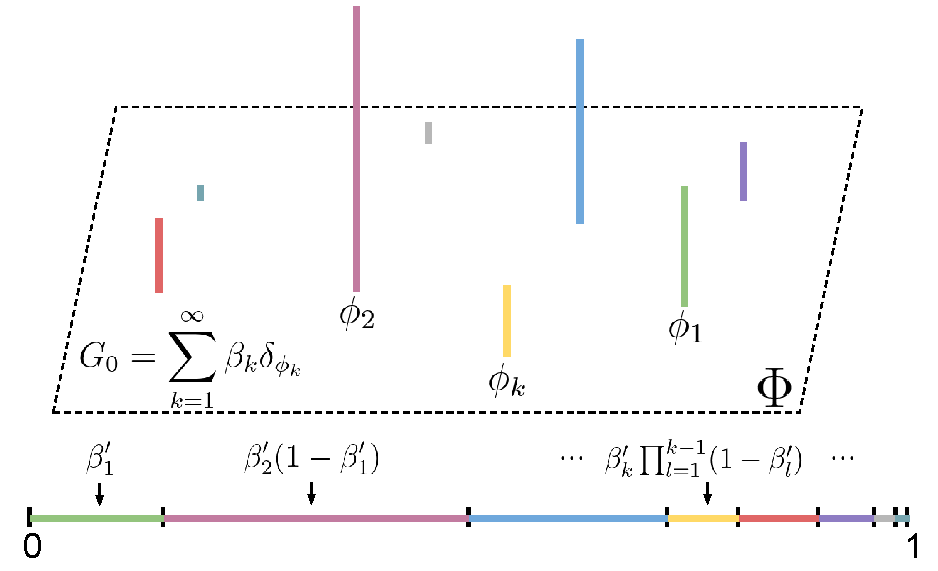
\includegraphics[trim=0cm 0cm 0cm 1cm, clip=true,width=0.8\linewidth]{figs/stick-breaking.pdf}
    \caption{Illustration of stick-breaking construction.}
    \label{fig:stick_breaking}
\end{figure}

In the mixture model context, we want to infer mixture components $\{\phi_{1}, \phi_{2}, \cdots, \phi_{k}, \cdots\}$ that fit to the data observations $\{x_{1}, x_{2}, \cdots, x_{n}\}$, which are assumed to be drawn from distributions $F(\phi)$ parameterized with variable $\phi$ (i.e., for a multivariate Gaussian $F$, $\phi = \{\mu, \Sigma\}$).
% We can now use DP to draw $\phi$ as $i$th mixture components corresponds to the $i$th observation $x_{i}$ by introducing the cluster assignment variable $y_{i} \sim \text{Mult}(\beta)$:
We now can use DP for drawing the component $\phi$ that corresponds to $x_{i}$ by introducing the cluster assignment variable $y_{i}\sim\text{Mult}(\beta)$:
\begin{equation}\label{eq:dpmm}
\begin{aligned}[c]
    \beta|\gamma &\sim \text{GEM}(\gamma) \\
    y_{i}|\beta &\sim \text{Mult}(\beta)
\end{aligned}
\qquad
\begin{aligned}[c]
    \phi_{k}|H &\sim H \\
    x_{i}|y_{i},\{\phi_{k}\} &\sim F(\phi_{y_{i}}) 
\end{aligned}
\end{equation}
where $\phi_{y_{i}}$ denotes the component parameter $\phi$ indexed by the assignment variable $y_{i}$ corresponding to the $i$th observation $x_{i}$.

\subsection{Hierarchical DPMM}\label{sec:hdpgmm:hdpmm}

In many data structures, groupings of atomic data points arise naturally (i.e., audio frames within a song, songs from an artist, words of lyrics). Hierarchical DP (HDP) is an extension of DP that models the ``groupings'' by imposing group-level DPs derived from the ``corpus-level'' DP as the global pool of components~\cite{doi:10.1198/016214506000000302}. Following~\cite{DBLP:journals/jmlr/WangPB11}, the $j$th group-level DP can be expressed as follows:
\begin{equation}\label{eq:hdp_doc_level}
\begin{aligned}[c]
    \pi^{\prime}_{jt} &\sim \text{Beta}(1, \alpha_{0}) \\
    \pi_{jt} &= \pi^{\prime}_{jt} \prod^{t - 1}_{s = 1} (1 - \pi^{\prime}_{js})
\end{aligned}
\qquad
\begin{aligned}[c]
    \psi_{jt} &\sim G_{0} \\
    G_{j} &= \sum^{\infty}_{t = 1} \pi_{jt}\delta_{\psi_{jt}}
\end{aligned}
\end{equation}
As seen above, HDP appears as the recursion of multiple levels of DPs\footnote{It implies naturally that multiple levels are possible (i.e., corpus - author - document) if it suits the data structure.}. Notably, the base distribution $G_{0}$ of each group-level DP is from the corpus-level DP. This relationship allows mapping group-level atoms $\psi_{jt}$ to the corpus-level atoms $\phi_{k}$. Wang et al.~\cite{DBLP:journals/jmlr/WangPB11} introduce indicator variables $c_{jt}\sim\text{Mult}(\beta)$ which maps $\psi_{jt}$ and $\phi_{k}$ by $\psi_{jt}=\phi_{c_{jt}}$, where $\beta$ is drawn from the corpus-level DP in Eq.\ (\ref{eq:stick_breaking}). It simplifies the model as we do not need to represent $\psi_{jt}$ explicitly.
Finally, we can represent HDPMM by introducing another indicator variable $z_{jn} \sim \text{Mult}(\pi_{j})$ for the $n$th observation $x_{jn}$ within the $j$th group, similarly to Eq.\ (\ref{eq:dpmm}):
\begin{equation}\label{eq:hdpmm}
\begin{aligned}[c]
    \pi_{j}|\alpha_{0} &\sim \text{GEM}(\alpha_{0}) \\
    z_{jn}|\pi_{j} &\sim \text{Mult}(\pi_{j})
\end{aligned}
\qquad
\begin{aligned}[c]
    \theta_{jn} = \psi_{jz_{jn}} &= \phi_{c_{jz_{jn}}}  \\
    x_{jn}|z_{jn}, c_{jt}, \{\phi_{k}\} &\sim F(\theta_{jn}) 
\end{aligned}
\end{equation}
where we use the indicator $z_{jn}$ to select $\psi_{jt}$, which eventually is mapped as $\phi_{c_{jz_{jn}}}$ that represents the parameter $\theta_{jn}$ to draw the observation $x_{jn}$. HDPGMM is then defined by simply setting $F$ as the (multivariate) Gaussian distribution and setting $H$ as one of the distributions from which we can sample the mean and covariance (i.e., Gaussian-inverse Wishart distribution). Figure \ref{fig:hdpmm} depicts the HDPGMM graphically.
\begin{figure}[ht]
    \centering
    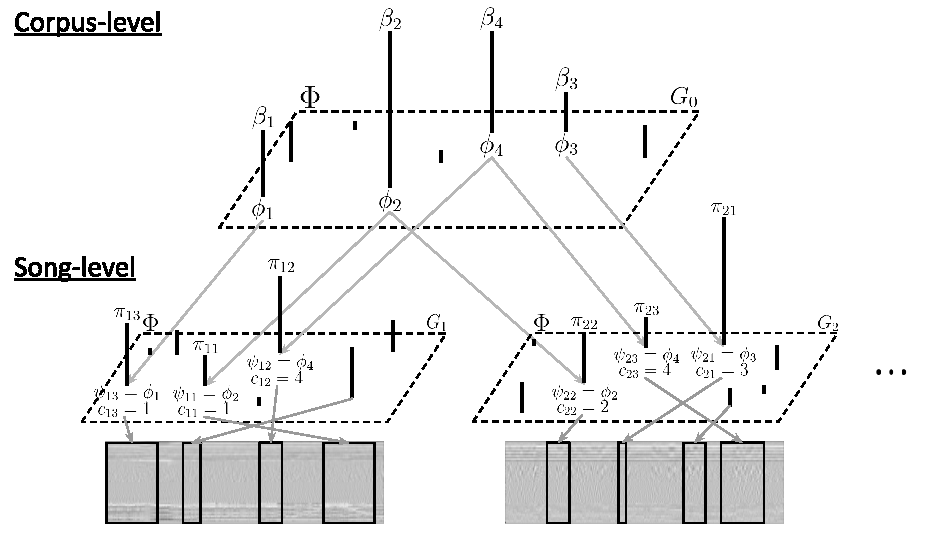
\includegraphics[width=\linewidth]{figs/HDP-stick-breaking.pdf}
    \caption{Illustration of 2-level HDPMM within corpus-song context. The top row depicts the corpus-level DP. The second row describes the draw of second-level (song-level) DPs per song from the corpus-level DP. Frame-level features are drawn from each song-level DPs, as depicted in the third row of the image.}
    \vspace{-0.4cm}
    \label{fig:hdpmm}
\end{figure}


\subsection{Inference Algorithm}\label{sec:hdpgmm:inference}

We employ the online Variational Inference (VI)~\cite{DBLP:journals/jmlr/WangPB11}, which is a common and significantly faster choice than the Markov Chain Monte Carlo (MCMC) method to infer fully Bayesian models. VI approximates the true posterior by minimizing the Kullback-Leibler (KL) divergence between the approximation $q(Z)$ and the true posterior $p(Z|X)$, where $Z$ denotes the set of latent variables and parameters that we want to find, and $X$ refers a set of observations~\cite{bishop2006pattern}.
One of the popular simplifications is the full factorization of the distribution $q(Z) = \prod^{|Z|}_{i=1} q_{i}(Z_{i})$. In the context of HDPGMM, we have the following factorization:
\begin{equation}\label{eq:meanfield_vi_hdpgmm}
    q(\beta^{\prime}, \pi^{\prime}, c, z, \phi) = q(\beta^{\prime})q(\pi^{\prime})q(c)q(z)q(\phi)
\end{equation}
where $\beta^{\prime}, \pi^{\prime}, c, z$ denote the corpus-level and group-level stick proportions, group-level component selection variable, and finally the observation-level component selection variable, respectively. $\phi$ refers to the parameter(s) for the $F$ which draws the atomic observation, set as (multivariate) Gaussian in our context. Thus, $\phi$ includes the means $\mu$ and precision matrices $\Lambda$ of each Gaussian component\footnote{We adopt the result from \cite{bishop2006pattern}, where the Gaussian-Wishart distribution is used for the prior.}.

Each variational distribution further factorizes into:
\begin{equation}\label{eq:meanfield_further}
\begin{aligned}[c]
    q(\beta^{\prime}) &= \textstyle \prod\nolimits_{k}^{K-1}\text{Beta}(\beta^{\prime}_{k}|u_{k}, v_{k}) \\
    q(\pi^{\prime}) &= \textstyle \prod\nolimits_{t}^{T-1}\text{Beta}(\pi^{\prime}_{t}|a_{t}, b_{t}) \\
    q(c) &= \textstyle \prod\nolimits_{j}\prod\nolimits_{t}\text{Mult}(c_{jt}|\varphi_{jt}) \\
    q(z) &= \textstyle \prod\nolimits_{j}\prod\nolimits_{n}\text{Mult}(z_{jn}|\zeta_{jn})
\end{aligned}
\end{equation}
where $u_{k}, v_{k}, a_{t}, b_{t}$ denote the variational parameters for the Beta distributions for corpus-level and group-level stick proportions, respectively. $\varphi_{jt}\in\mathbb{R}^{K}, \zeta_{jn}\in\mathbb{R}^{T}$ are the variational parameters for the Multinomial distribution to draw the selector $c$ and $z$. Also, we truncate the infinite Beta distributions by $K$ and $T$, which is a common way to avoid actually computing the infinite dimension~\cite{DBLP:journals/jmlr/WangPB11}. With a sufficiently large number for the truncation, the model will still not be limited to the truncation and will only use the number of components optimal for the dataset. The final variational distribution is the Gaussian-Wishart distribution which draws the Gaussian parameters $\phi$ for $F$:
\begin{equation}\label{eq:meanfield_normalwishart}
    q(\phi) = \textstyle \prod\nolimits_{k}^{K}\mathcal{N}(\mu_{k}|m_{k}, (\lambda_{k}\Lambda_{k})^{-1})\mathcal{W}(\Lambda_{k}|W_{k}, \nu_{k})
\end{equation}
where we draw the precision $\Lambda_{k}\in\mathbb{R}^{d \times d}$ from the Wishart distribution with the variational parameter $W_{k}\in\mathbb{R}^{d \times d}$ and $\nu_{k}\in\mathbb{R}$, and the mean $\mu_{k}\in\mathbb{R}^{d}$ is drawn by the precision weighted by $\lambda_{k}\in\mathbb{R}$ and mean $m_{k}\in\mathbb{R}^{d}$.

We then can obtain the optimal model by maximizing the lower bound of the marginal log likelihood $\text{log}\,p(X|Z)$~\cite{bishop2006pattern, DBLP:journals/ml/JordanGJS99, 10.1214/06-BA104}:
\begin{equation}\label{eq:lowerbound}
\begin{aligned}
    \text{log}\, p(X|Z) \geq \mathbb{E}_{q}[\text{log}\,p(X, \beta^{\prime}, \pi^{\prime}, c, z, \phi)] + H(q) \\
    = \textstyle \sum_{j} \big\{ \mathbb{E}_{q}[\text{log}\,(p(X_{j}|c_{j}, z_{j}, \phi)p(c_{j}|\beta^{\prime})p(z_{j}|\pi_{j}^{\prime})p(\pi^{\prime}_{j}|\alpha_{0}))] \\
    + H(q(c_{j})) + H(q(z_{j})) + H(q(\pi^{\prime}_{j})) \big\} \\
    + \mathbb{E}_{q}[\text{log}\,p(\beta^{\prime})p(\phi)] + H(q(\beta^{\prime})) + H(q(\phi))
\end{aligned}
\end{equation}
where $H(\cdot)$ denotes the entropy of given distribution, and $X_{j} = \{x_{j1}, x_{j2}, \cdots, x_{jN_{j}}\}$ is a set of observations within the $j$th group.\footnote{
% Thus, the terms inside the sum over the group would further factorize into sums of these per-group observation. We omit them to avoid the equation being too crammed.
Thus, the terms inside the sum over the group would further factorize into sums of per-group observations. We do not write these out for legibility and space considerations.
}

Using the standard result of VI~\cite{bishop2006pattern, 10.1214/06-BA104, DBLP:journals/jmlr/WangPB11}, the update rules for group-level parameters are derived as follows:
\begin{align}
\label{eq:doc_update:a} a_{jt} &= \textstyle 1 +  \sum_{n}\zeta_{jnt} \\
\label{eq:doc_update:b} b_{jt} &= \textstyle \alpha_{0} +  \sum_{n}\sum^{T}_{s=t+1}\zeta_{jns} \\
\label{eq:doc_update:varphi} \varphi_{jtk} &\propto \text{exp}(\textstyle \sum_{n}\zeta_{jnt}\mathbb{E}_{q}[\text{log}\,p(x_{jn}|\phi_{k})] + \mathbb{E}_{q}[\text{log}\,\beta_{k}]) \\
\label{eq:doc_update:zeta} \zeta_{jnt} &\propto \text{exp}(\textstyle \sum_{k=1}^{K} \varphi_{jtk} \mathbb{E}_{q}[\text{log}\,p(x_{jn}|\phi_{k})] + \mathbb{E}_{q}[\text{log}\,\pi_{jt}])
\end{align}
Similarly, the update rules for the corpus-level parameters are as follows~\cite{bishop2006pattern}:
\begin{align}
\label{eq:corpus_update:u} u_{k} &= 1 + \textstyle \sum_{j}\sum_{t=1}^{T} \varphi_{jtk} \\
\label{eq:corpus_update:v} v_{k} &= \gamma + \textstyle \sum_{j}\sum_{t}^{T}\sum_{l=k+1}^{K} \varphi_{jtl} \\
\label{eq:corpus_update:lambda} \lambda_{k} &= \lambda_{0} + N_{k} \\
\label{eq:corpus_update:m} m_{k} &= \lambda_{k}^{-1} (\lambda_{0}m_{0} + N_{k}\bar{x}_{k}) \\
\label{eq:corpus_update:W} W_{k}^{-1} &= W_{0}^{-1} + N_{k}S_{k} + \frac{\lambda_{0}N_{k}}{\lambda_{0} + N_{k}} (\bar{x}_{k} - m_{0})(\bar{x}_{k} - m_{0})^{\intercal} \\
\label{eq:corpus_update:nu} \nu_{k} &= \nu_{0} + N_{k}
\end{align}
where $\lambda_{0}\in\mathbb{R}, m_{0}\in\mathbb{R}^{d}, \nu_{0}\in\mathbb{R}, W_{0}\in\mathbb{R}^{d\times d}$ are the hyperparameters corresponding to the weight, location, degrees of freedom, and scale of Gaussian-Wishart distribution. The ``sufficient statistics'' and expectations in the update rules are defined as follows:
\begin{align}\label{eq:expectations_and_suffstats}
    &\mathbb{E}_{q}[\text{log}\,\beta_{k}] = \mathbb{E}_{q}[\text{log}\,\beta_{k}^{\prime}] + \textstyle\sum_{l=1}^{k-1}\,\mathbb{E}_{q}[\text{log}\,(1 - \beta_{l}^{\prime})] \nonumber\\
    &\mathbb{E}_{q}[\text{log}\,\beta_{k}^{\prime}] = \Psi(u_{k}) - \Psi(u_{k} + v_{k}) \nonumber\\
    &\mathbb{E}_{q}[\text{log}\,(1 - \beta_{k}^{\prime})] = \Psi(v_{k}) - \Psi(u_{k} + v_{k}) \nonumber\\
    &\mathbb{E}_{q}[\text{log}\,\pi_{jt}] = \mathbb{E}_{q}[\text{log}\,\pi_{jt}^{\prime}] + \textstyle\sum_{s=1}^{t-1}\,\mathbb{E}_{q}[\text{log}\,(1 - \pi_{s}^{\prime})] \nonumber\\
    &\mathbb{E}_{q}[\text{log}\,\pi_{jt}^{\prime}] = \Psi(a_{jt}) - \Psi(a_{jt} + b_{jt}) \nonumber\\
    &\mathbb{E}_{q}[\text{log}\,(1 - \pi_{jt}^{\prime})] = \Psi(b_{jt}) - \Psi(a_{jt} + b_{jt}) \nonumber\\
    &N_{k} = \textstyle\sum_{j}\sum_{n}\,r_{jnk} \nonumber\\
    &\bar{x}_{k} = \frac{1}{N_{k}}\textstyle\sum_{j}\sum_{n}\,r_{jnk}x_{jn} \nonumber\\
    &S_{k} = \frac{1}{N_{k}}\textstyle\sum_{j}\sum_{n}\,r_{jnk}(x_{jn} - \bar{x}_{k})(x_{jn} - \bar{x}_{k})^{\intercal} \nonumber
\end{align}
where $\Psi(\cdot)$ refers to the digamma function, and $r_{jnk} = \sum_{t=1}^{T} \zeta_{jnt}\varphi_{jtk}$ is the inferred ``responsibility'' of the $n$th observation of the $j$th group on the $k$th component. A standard batch update would compute statistics across the entire corpus, and update the corpus-level parameters. However, it may be slow or may suffer from too large or small numbers accumulated from a large-scale corpus.

We therefore employ the online VI, where corpus-level parameters are updated per mini-batch of groups passed. In this way, the early phase of model inference can be accelerated substantially compared to the full-batch update~\cite{DBLP:journals/jmlr/WangPB11, DBLP:conf/nips/HoffmanBB10}. The corpus-level update is then controlled by the learning rate $\rho_{t} = (\tau_{0} + t)^{-\kappa}$, which is decayed over iterations parameterized by the offset $\tau_{0} > 0$ and the rate $\kappa \in (0.5, 1]$:
\begin{equation}\label{eq:minibatch_update}
    Z_{t} = (1 - \rho_{t})Z_{t - 1} + \rho_{t}\tilde{Z}_{t}
\end{equation}
where $\tilde{Z}_{t}$ denotes one of the corpus-level parameters from \crefrange{eq:corpus_update:u}{eq:corpus_update:nu}, which is updated by the given mini-batch at $t$th iteration, while $Z_{t-1}$ is the current parameter. To scale the update with respect to the mini-batch size, we weight $\tilde{Z}$ by the factor of $w = \frac{|\tilde{X}|}{|X|}$, where $|X|, |\tilde{X}|$ denote the number of groups within the entire observation set $X$ and the mini-batch of groups $\tilde{X}$. The overall inference algorithm is described in Algorithm \ref{alg:inference}.

\begin{algorithm}
\small
\caption{Online VI for HDPGMM}\label{alg:inference}
Initialize $\mathbf{\phi}=(\phi_{k})^{K}_{k=1}$, $u=(u_{k})^{K}_{k=1}$, $v=(v_{k})^{K}_{k=1}$ randomly. Set $t=1$.\\
\While{Stopping criterion is not met}{
    Fetch a random mini-batch of groups $\tilde{X}$ \\
    \Repeat{mini-batch likelihood stops improving}{
        Update $a_{j}, b_{j}, \zeta_{j} \text{and} \varphi_{j}$ using \crefrange{eq:doc_update:a}{eq:doc_update:zeta}\\
    }
    Compute $u_{k}, v_{k}, \lambda_{k}, m_{k}, W_{k}, \text{and } \nu_{k}$ using \crefrange{eq:corpus_update:u}{eq:corpus_update:nu} \\
    Set $\rho_{t} = (\tau_{0} + t)^{-\kappa}$, $t \gets t + 1$ \\
    Update $u_{k}, v_{k}, \lambda_{k}, m_{k}, W_{k}, \text{and} \nu_{k}$ using Eq. (\ref{eq:minibatch_update})
}
\end{algorithm}

% \subsection{Further Regularization}\label{sec:hdpgmm:regularization}

Inspired by the implementation of \cite{DBLP:journals/jmlr/WangPB11, 10.1214/06-BA104}, we apply further regularization to the model. Specifically, we ``splash'' the uniform noise to the inferred responsibility $r_{jn}$ as it can be biased if the groups are corrupted or incomplete, such as the preview audio of the entire song:
\begin{equation}\label{eq:additional_regularization}
    \tilde{r}_{jn} = (1 - \eta_{t}) r_{jn} + \eta_{t} e
\end{equation}
$\eta_{t}$ is the regularization coefficient that determines the extent uniform noise $e = (e_{k})_{k=1}^{K}$ is mixed into $r_{jn}$. $\eta_{t} = \frac{\eta_{0} * 10^{3}}{(t + 10^{3})}$ also is defined as decaying function similar to the learning rate $\rho_{t}$.


% \subsection{DPMMs in MIR}\label{sec:hdpgmm:in_mir}

%blahblah


\section{Experimental Setup}\label{sec:experimental_setup}

This section discusses the details of the experiment. The overall design is adopted from the recent music representation learning studies~\cite{DBLP:conf/ismir/ChoiFSC17,DBLP:journals/nca/KimULH20,DBLP:conf/ismir/SpijkervetB21}, where multiple downstream MIR tasks are tested with the feature set learned from the representation models.

\subsection{Datasets, Features \& Evaluation}\label{sec:experimental_setup:datasets_evaluation}

We use a subset of Million Song Dataset (\textbf{MSD})~\cite{Bertin-Mahieux2011} as the dataset for the representation learning; more specifically, the audio preview excerpts from the MSD ``train'' subset introduced by~\cite{DBLP:conf/ismir/PonsNPSES18,app8010150}\footnote{Length of preview audio differs per clip, where about 70\% of samples are approximately 30 seconds and the rest are 1 minute, with a small subset is longer than 1 minute.}.
For the evaluation of the representation, we employ three downstream tasks encompassing \emph{music genre classification}, \emph{music auto tagging}, and  \emph{music recommendation}. For each target task, we chose the \textbf{GTZAN} dataset~\cite{DBLP:journals/taslp/TzanetakisC02} with the fault-filtered split~\cite{DBLP:journals/tmm/KereliukSL15}, the MagnaTagaTune (\textbf{MTAT}) dataset~\cite{DBLP:conf/ismir/LawWMBD09} with the split from ~\cite{lee_multi-level_2017}, and finally the Echo Nest taste profile subset as part of MSD (\textbf{Echonest})~\cite{Bertin-Mahieux2011} filtered by user and item frequency~\cite{DBLP:conf/www/LiangKHJ18}.

We evaluate the modeling using the cross-validation of task-specific prediction models. We fit the logistic regression models for the GTZAN and MTAT datasets, taking learned music representation as input and predicting the genre or music tags. We find the hyper-parameters of the logistic regression model by the randomized parameter search~\cite{DBLP:journals/jmlr/BergstraB12} for each run. As for the recommendation, we apply the item \emph{K} Nearest Neighbor (\emph{item-kNN}) method~\cite{DBLP:journals/tois/DeshpandeK04} where the song-song similarity is measured by the \emph{cosine similarity} of the learned music representation. We adopt the data split introduced in \cite{DBLP:conf/www/LiangKHJ18}. For every trial, disjoint validation and test users are uniformly sampled, which includes $1142$ users for each. Then $30\%$ of listening records of these users are held out as testing records. We find the best \emph{K} by conducting the grid search on the range $\textit{K}\in\{2^{4}, 2^{5}, 2^{6}, 2^{7}, 2^{8}, 2^{9}\}$ by measuring the accuracy on the validation users. Using the best \emph{K}, we compute the final score on the held out test records of testing users. We take the average score over $5$ repetitions for each run to incorporate the random split effect.

We repeat $5$ evaluation ``runs'' for each learning trial to consider the various random effects (i.e., initialization, randomized search). We employ the commonly used accuracy measures in each task to assess them,  which are further elaborated in Table~\ref{tab:dataset}.

\begin{table}[h!]
\centering
\small
\begin{tabular}{ cccc }
    \hline
    Id       & \# Samples & \# Classes/\# Users   & Acc. Measure \\ 
    \hline
    \hline 
    MSD      & $213,354$ & N/A           & N/A          \\ 
    \hline
    GTZAN    & $1,000$   & $10$          & F1~\cite{DBLP:books/bu/Rijsbergen79} \\
    MTAT     & $25,863$  & $50$          & AUROC~\cite{DBLP:journals/prl/Fawcett06} \\
    Echonest & $40,980$  & $571,355$\tablefootnote{It refers the number of users in this dataset.} & nDCG~\cite{DBLP:journals/tois/JarvelinK02} \\
    \hline
\end{tabular}
\caption{Details on the datasets. We use \emph{macro} average strategy for F1 and Area Under Receiver Operating Characteristic curve (AUROC) measure, and we consider the top $500$ recommended songs for computing the normalized Discounted Cumulative Gain (nDCG).}
\vspace{-0.3cm}
\label{tab:dataset}
\end{table}

We select a set of audio features to infer the HDPGMM and non-DL baseline models inspired by~\cite{DBLP:journals/taffco/WangLCCH15}. The detailed curation of the features can be found in Table~\ref{tab:feature}\footnote{We use the implementation of \texttt{librosa}~\cite{librosa_0_9_1} with the default parameters for all the features.}.

\begin{table}[h!]
\centering
\small
\begin{tabular}{ cccc }
    \hline
    Feature       & Aspect   & Dim.   & Transform\\ 
    \hline
    \hline 
    MFCC & Timbre & 13 & -         \\ 
    $\Delta$MFCC & Timbre & 13 & -         \\ 
    $\Delta\Delta$MFCC & Timbre & 13 & -         \\ 
    Onset Strength\cite{88} & Rhythm & 1 & $\text{log}$  \\ 
    Chroma\cite{ellis_2007} & Tonal & 12 & $\text{log}$  \\ 
    \hline
\end{tabular}
\caption{Details on the base audio features we employed for the experiment.}
\vspace{-0.2cm}
\label{tab:feature}
\end{table}

\subsection{Comparisons}\label{sec:experimental_setup:comparisons}

We evaluate $4$ comparisons against HDPGMM, including DL-based and non-DL-based models.

\begin{itemize}[noitemsep, leftmargin=*]
    \item \textbf{G1} is the simplest model among the comparisons. The song-wise feature is represented by the concatenated parameters $\phi = \{\mu, \Sigma\}$ of the single multivariate Gaussian fitted on the frame-level base audio feature vectors within a song\footnote{We chose the diagonalized covariance, which means the feature is the concatenation of \emph{mean} $\mu\in\mathcal{R}^{52}$ and \emph{standard deviation} $\sigma\in\mathcal{R}^{52}$ of features.}.

    \item \textbf{VQ Codebook} can be deemed as the approximation of HDPGMM models~\cite{DBLP:conf/ismir/HoffmanBC08}. First, a corpus-wise $K$-means clustering is fitted on the frame level features. Later song-level feature is represented by the normalized frequency of cluster assignment of each frame-level feature within the song\footnote{It can be interpreted similarly to the inferred cluster assignment variable $\pi_{j}$ in Eq. (\ref{eq:hdpmm})}. We set $K=256$.

    \item \textbf{KIM} is a DL-based music representation trained in a simple self-supervised learning framework with a \emph{VGG-like}~\cite{DBLP:journals/corr/SimonyanZ14a} architecture~\cite{DBLP:journals/nca/KimULH20}.
    % The objective function of the model is to measure the extent to which a \emph{VGG-like} based Siamese network~\cite{DBLP:journals/corr/SimonyanZ14a, koch2015siamese} can predict whether the two input clips are cropped from the same song or different songs.
    We use the original implementation of the work, which takes the stereo mel-spectrogram of a $2.5$ second-length clip as input. The representation is extracted from the last hidden layer before the prediction and summarized with global average and standard deviation pooling through the entire song.

    \item \textbf{CLMR}~\cite{DBLP:conf/ismir/SpijkervetB21} is a recent DL-based music representation employing self-supervised learning through the contrastive learning method~\cite{DBLP:conf/icml/ChenK0H20}. We employ the original implementation of~\cite{DBLP:conf/ismir/SpijkervetB21} that uses the $2.67$ second-length raw audio samples as input feature\footnote{Unlike the original work, we reduce the dimensionality of the hidden layer, from which we extract the representation, from $512$ to $256$ to control the representation dimensionality with other comparisons. Also, we do not apply the data augmentation for a fair comparison and also as it is beyond the main scope of the work. However, as it is reported that it can meaningfully improve the representation, we assume that applying the method would benefit similarly to other models as well.}. The representation is drawn from the last hidden layer and pooled with the global average over the entire song excerpt.

    \item \textbf{HDPGMM}\footnote{inference algorithm in \Cref{alg:inference} is implemented on \texttt{PyTorch}~\cite{NEURIPS2019_9015}, and thus supports the GPU acceleration.} uses the base audio feature with the whitening following~\cite{DBLP:conf/ismir/NamHSS12}. As for song-level representation $y_{j}$, we employ the  exponentiation of the expectation $\tilde{y}_{jk} = \text{exp}(\mathbb{E}_{q}[\text{log}\,p(X_{j}|c_{j}, z_{j}, \phi_{k})])$ and normalize them over components and the length of the clip $y_{jk} = N_{j}^{-1}\frac{\tilde{y}_{jk}}{\sum_{k^{\prime}=1}^{K}\tilde{y}_{jk^{\prime}}}$. We adopt many hyper-parameter setups from the result of~\cite{DBLP:journals/jmlr/WangPB11}; we set the truncation of components on the corpus level $K$ and the song level $T$ as $256$ and $32$ respectively, mini-batch size to $1024$, learning rate parameters $\kappa=0.6$ and $\tau_{0}=64$. We, however, explore the regularization rate $\eta_{0} \in \{10^{-4}, 10^{-3}, 10^{-2}, 10^{-1}\}$ and total corpus size $|X| \in \{2\times10^{3}, 2\times10^{4}, 213354\}$ to examine their effect on the representation.
\end{itemize}

For all the comparisons except G1, we repeat $3$ learning trials to incorporate any random effect of learning algorithms. Within a trial, we iterated the update for $100$ epochs for KIM, CLMR, and HDPGMM. Further, we set the representation's dimensionality to $256$, homogeneous across all comparisons except $G1$. Finally, we take the logarithm of the representation $\hat{y_{j}} = \text{log}(\text{max}(y_{j}, 10^{-8}))$ if it is given as the probability simplex (i.e., VQCodebook, HDPGMM).


\section{Result and Discussion}\label{sec:result_discussion}

\subsection{Effect of Learning Factors}\label{sec:result_discussion:learning_factors}

Overall, we observe that the learning factors of HDPGMM can make a substantial difference. As Figure \ref{fig:effects} shows, the result suggests that the additional regularization in Eq. (\ref{eq:additional_regularization}) generally affects positively the performance of all the downstream tasks we tested. It implies that the entire song inputs would likely improve the representation further, as the regularization crudely masks the effect of the missing data due to the preview clipping to some extent.

Further, we find that the number of training samples positively affects the performances in general. We measured the effect by repeatedly sub-sampling the MSD training data $5$ times in two different sizes mentioned in \ref{sec:experimental_setup:comparisons}, and conducted the same evaluation routine applied for the full training set. The result shows that the positive effect is logarithmic, which suggests that the model should be learned with an exponentially larger dataset to get a linear improvement in the performance. The recommendation task, on the other hand, indicates the effect may not be linear, as we observe that the learning with $2\times10^{3}$ samples outperforms the $2\times10^{4}$ samples. However, the largest dataset leads to a better representation than the smallest datasets.
\begin{figure}[h]
    \begin{subfigure}{\linewidth}    
        \centering
        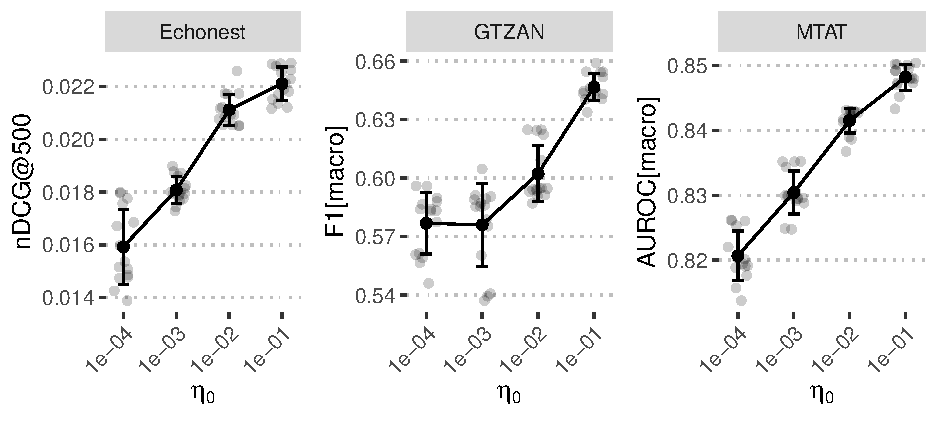
\includegraphics[width=\linewidth]{figs/regularization_effect.pdf}
        \caption{Effect of regularization factor $\eta_{0}$. ($|X| = 213,354$)}
        \label{fig:effects:regularization_effect}
    \end{subfigure}

    \begin{subfigure}{\linewidth}
        \centering
        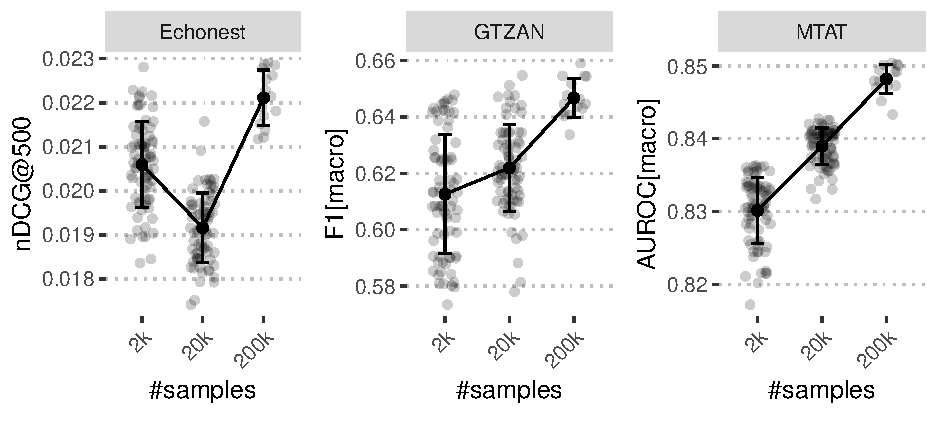
\includegraphics[width=\linewidth]{figs/num_sample_effect.pdf}
        \caption{Effect of the number of training samples. ($\eta_{0} = 10^{-1}$)}
        \label{fig:effects:num_samples_effect}
    \end{subfigure}
    \caption{Effect of the learning factors on HDPGMM. The error bar indicates the standard deviation, and grey dots are the raw data points.}
    \vspace{-0.3cm}
    \label{fig:effects}
\end{figure}

\subsection{Model Comparison}\label{sec:result_discussion:model_comparison}

\begin{table}[h]
\small
\centering
\begin{tabular}{ c|c|l|c }
    \hline
    Dataset                 & Measure              & Model         & Mean ($\pm$SD)    \\ 
    \hline
    \hline 
    \multirow{5}*{Echonest} & \multirow{5}*{nDCG}  & G1            & 0.0237 ($\pm$ 0.0011) \\ 
                            &                      & VQCodebook    & 0.0155 ($\pm$ 0.0003) \\
                            &                      & KIM           & 0.0257 ($\pm$ 0.0015) \\
                            &                      & CLMR          & \textbf{0.0362 ($\pm$ 0.0012)} \\
                            &                      & HDPGMM        & 0.0221 ($\pm$ 0.0006) \\
    \hline
    \multirow{5}*{GTZAN}    & \multirow{5}*{F1}    & G1            & 0.5396 ($\pm$ 0.0049) \\ 
                            &                      & VQCodebook    & 0.5777 ($\pm$ 0.0022) \\
                            &                      & KIM           & 0.5420 ($\pm$ 0.0290) \\
                            &                      & CLMR          & \textbf{0.6375 ($\pm$ 0.0368)} \\
                            &                      & HDPGMM        & \textbf{0.6467 ($\pm$ 0.0069)} \\
    \hline
    \multirow{5}*{MTAT}     & \multirow{5}*{AUROC} & G1            & 0.8441 ($\pm$ 0.0006) \\ 
                            &                      & VQCodebook    & 0.8386 ($\pm$ 0.0013) \\
                            &                      & KIM           & 0.8014 ($\pm$ 0.0045) \\
                            &                      & CLMR          & 0.8262 ($\pm$ 0.0026) \\
                            &                      & HDPGMM        & \textbf{0.8482 ($\pm$ 0.0020)} \\
    \hline
\end{tabular}
\caption{Evaluation results on downstream tasks.}
\vspace{-0.3cm}
\label{tab:main_result}
\end{table}

% \begin{table*}[h]
\begin{table*}[hbt!]
\centering
\small
\begin{tabular}{ ccccccc }
    \hline
    Hip-Hop & country & female vocalists & pop & electronic & pop & oldies \\
    pop & rock & singer-songwriter & female vocalists & dance & soul & blues \\
    rnb & pop & pop & female vocalist & electronica & female vocalists & country \\
    soul & oldies & acoustic & rock & funk & rnb & 60s \\
    male vocalists & indie & Mellow & Love & electro & dance & soul \\
    rock & singer-songwriter & folk & dance & Hip-Hop & Hip-Hop & rock \\
    % hip hop & classic rock & female vocalist & female & House & rock & classic rock \\
    \hline
    $0.0394$ & $0.0308$ & $0.0299$ & $0.0269$ & $0.0268$ & $0.0248$ & $0.0227$ \\
    \hline
\end{tabular}
\caption{Top tags for a few mostly ``loaded'' components (column-wise). The last row is the normalized total responsibility $\tilde{N}_{k} = \frac{N_{k}}{\sum_{k^{\prime}}^{K} N_{k^{\prime}}}$, meaning the proportional amount of songs having the component.}
\vspace{-0.3cm}
\label{tab:topic_tags}
\end{table*}

Model comparison suggests that the HDPGMM model is comparable to the DL representation on average and can outperform in a few specific scenarios. For the comparison, we chose the best HDPGMM model according to the result in \ref{sec:result_discussion:learning_factors} by setting $\eta_{0}=10^{-1}$ and using the entire dataset. As reported in Table \ref{tab:main_result}, KIM achieves worse performance than HDPGMM on GTZAN and MTAT while better at recommendation (Echonest). On the other hand, CLMR, which adopts a more sophisticated learning strategy, achieves the best performance in Echonest, but worse than HDPGMM on the MTAT and comparable on the GTZAN. It is notable that the mixture model variants (VQCodebook, HDPGMM) perform particularly worse in the recommendation task. We hypothesize that the cosine similarity might not be an optimal choice for the probability simplex representation, or the feature set we consider may lack aspects that are crucial for the recommendation; this requires further study.

Except for this corner case, the HDPGMM representation outperforms the other non-DL comparisons in general. It especially achieves significant improvement over its simplified version (VQCodebook) for all tasks, and mostly outperforms G1.


\subsection{Component Interpretability}\label{sec:result_discussion:interpretability}

Finally, we explore the interpretability aspect of the HDPGMM model. To achieve it, we employ the \emph{Lastfm-MSD} music tag dataset~\cite{Bertin-Mahieux2011} where we find the mapping between the MSD songs and the social music tags. All our MSD training samples have mappings to the social tags, whose vocabulary size reaches roughly half a million. We compute the most relevant music tags for each corpus-level component found by the HDPGMM model. We estimate the relevance by a proxy measure $\alpha_{tk} = \sum_{j\in{X}:t\in{j}}N_{j}^{-1}\sum_{n}r_{jnk}$, where $t$ denotes the tag index and $r_{jnk}$ refers the responsibility computed in Eq. (\ref{eq:additional_regularization})\footnote{To improve the clarity and interpretability, we filter the most popular tags by weighting the measure by the Inverse Document Frequency (IDF) for each tag.}. Table \ref{tab:topic_tags} shows an example from one of the HDPGMM with high regularization ($\eta_{0}=10^{-1}$). It suggests that the most frequent component (the first column) can be interpreted as the corpus-wide, universal topic. From second to the rest it represents a few other topics of music, such as \emph{country-rock (column 1)}, \emph{pop-female vocalist (column 2, 3, 5)}, and \emph{electronic-dance (column 4)}. Notably, several compatible topics (i.e., columns 2, 3, and 5) exist, which can be interpreted as the collection of slightly different sub-clusters of an umbrella topic. It suggests that the advanced BN methods such as the hierarchical latent component models using the nested HDP~\cite{DBLP:journals/pami/PaisleyWBJ15} would further improve the representation.


\section{Conclusion and Future Works}\label{sec:conclusion}

In this work, we explore the potential of a BN model in the MIR task space.
% We assess the effectiveness of representation learned from the HDPGMM applied in a range of MIR downstream tasks compared to the DL-based representations.
The results suggest that the HDPGMM representation achieves comparable effectiveness over the DL equivalents and outperforms a few scenarios. It implies that the method can be as effective as DL models when used in the supervised learning setup as well, by, for instance, jointly maximizing the variational lower bound both for the data generation and the prediction tasks. It has already been shown that such a joint objective approach can outperform the separated feature learning and transfer strategy that we demonstrate in this work~\cite{DBLP:journals/taffco/WangLCCH15}.

Notably, HDPGMM is one of the more simple models in the BN approach. As mentioned above, there are models that are ``deeper'' such as nested DP models, which allow for a hierarchical structure of latent components~\cite{DBLP:journals/pami/PaisleyWBJ15}. The model also can be improved by introducing a sequential model such as Hidden Markov Models (HMM) as a base distribution~\cite{DBLP:conf/icassp/QiPC07}, as the HDPGMM model assumes the exchangeability of tokens (feature frames), which is not ideal for a music signal.
% Also, we show that the model can handle a decent scale of the dataset with an efficient implementation employing accelerations such as GPU. We believe that the implementation can be further improved for faster inference, which would allow the bigger model and datasets and longer inferences for better convergence.

% For bibtex users:
\bibliography{ISMIRtemplate}

\end{document}

